\subsection{MLPerf HPC - OpenFold}
{{\footnotesize
\noindent MLPerf HPC introduces scientific model benchmarks (e.g., CosmoFlow, DeepCAM) aimed at large-scale HPC evaluation with >10x performance scaling through system-level optimizations.


\begin{description}[labelwidth=4cm, labelsep=1em, leftmargin=4cm, itemsep=0.1em, parsep=0em]
  \item[date:] 2021-10-20
  \item[version:] v1.0
  \item[last\_updated:] 2021-10
  \item[expired:] unknown
  \item[valid:] yes
  \item[valid\_date:] 2021-10-20
  \item[url:] \href{https://github.com/mlcommons/hpc}{https://github.com/mlcommons/hpc}
  \item[doi:] 10.48550/arXiv.2110.11466
  \item[domain:]
    - Biology \& Medicine
  \item[focus:] Scientific ML training and inference on HPC systems
  \item[keywords:]
    - HPC
    - training
    - inference
    - scientific ML
  \item[licensing:] Apache License 2.0
  \item[task\_types:]
    - Training
    - Inference
  \item[ai\_capability\_measured:]
    - Scaling efficiency
    - training time
    - model accuracy on HPC
  \item[metrics:]
    - Training time
    - Accuracy
    - GPU utilization
  \item[models:]
    - DeepCAM
  \item[ml\_motif:]
    - Sequence Prediction/Forecasting
  \item[type:] Framework
  \item[ml\_task:]
    - NA
  \item[solutions:] Solution details are described in the referenced paper or repository.
  \item[notes:] Shared framework with MLCommons Science; reference implementations included.

  \item[contact.name:] Steven Farrell (MLCommons)
  \item[contact.email:] unknown
  \item[results.links.name:] ChatGPT LLM
  \item[fair.reproducible:] Yes
  \item[fair.benchmark\_ready:] Yes
  \item[id:] mlperf\_hpc\_-\_openfold
  \item[Citations:] \cite{farrell2021mlperfhpcholisticbenchmark}
\end{description}

{\bf Ratings:} ~ \\

\begin{tabular}{p{0.15\textwidth} p{0.07\textwidth} p{0.7\textwidth}}
\hline
Rating & Value & Reason \\
\hline
dataset & 5 & Not all data is independently versioned or comes with standardized FAIR metadata.
 \\
documentation & 4 & Central guidance is available but requires domain-specific effort to replicate results across systems.
 \\
metrics & 5 & None
 \\
reference\_solution & 4 & Reproducibility and environment tuning depend on system configuration; baseline models not uniformly bundled.
 \\
software & 3 & Reference implementations exist but containerization and environment setup require manual effort across HPC systems.
 \\
specification & 4 & Hardware constraints and I/O formats are not fully defined for all scenarios.
 \\
\hline
\end{tabular}

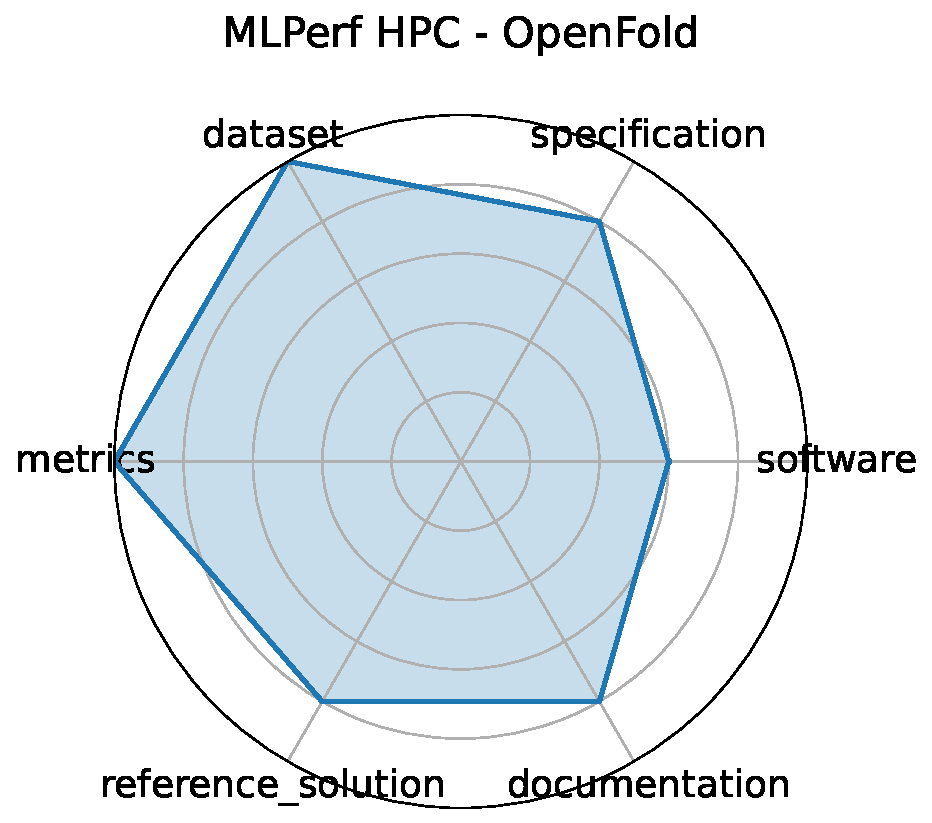
\includegraphics[width=0.2\textwidth]{mlperf_hpc_-_openfold_radar.pdf}
}}
\clearpage